% Copyright 2019 Clara Eleonore Pavillet

% Author: Clara Eleonore Pavillet
% Description: This is an unofficial Oxford University Beamer Template I made from scratch. Feel free to use it, modify it, share it.
% Version: 1.0
% \documentclass[xcolor=table]{beamer}
\documentclass{beamer}
\usepackage[version=4]{mhchem}
\usepackage{lipsum}  % Generates filler text
\usepackage[export]{adjustbox}
% Load Packages
\usepackage[utf8]{inputenc}
\usepackage{xcolor}
\usepackage{tikz}
\usetikzlibrary{positioning,calc}
\usepackage{graphicx}
\usepackage{hyperref}
\usepackage{amsmath}
\usepackage{listings}
\usepackage{fontawesome}

% Define Commands
\newcommand*{\ClipSep}{0.06cm} %To adjust footer logo
\newcommand{\E}{\mathrm{e}\,} %\def\I{e} % used to defined e for exp(x), see later what it should be
\newcommand{\ud}{\mathrm{d}}
\lstset{numbers=left, numberstyle=\tiny, stepnumber=1,firstnumber=1,breaklines=true,
    numbersep=5pt,language=Python,
    stringstyle=\ttfamily,
    basicstyle=\footnotesize, 
    showstringspaces=false
}

% ----- ----- ----- ----- ----- ----- -----
% Miscellaneous
\usepackage{pdfsync}  % enable references between source and PDF
\usepackage[utf8]{inputenc}  % allows for unicode (UTF8) not just ASCII source
\usepackage{xcolor}  % advanced colors
\usepackage{setspace}  % control spacing between lines
\usepackage{listings}  % typesetting code
\usepackage[normalem]{ulem}  % underlining
\usepackage{subfiles}  % enable subfiles to be able to run standalone

% ----- ----- ----- ----- ----- ----- -----
% Floats
\usepackage{caption}  % advanced captions
\usepackage{rotating}  % rotate floats

% ----- ----- ----- ----- ----- ----- -----
% Graphics
\usepackage{graphicx}  % including graphics
\usepackage{pdfpages}  % including external pdfs
\usepackage{pgfgantt}  % Gantt charts

% ----- ----- ----- ----- ----- ----- -----
% Math
\usepackage{amsmath}  % features for mathematical typesetting
\usepackage{amsfonts}  % extended fonts for mathematics
\usepackage{amssymb}  % extended symbols
\usepackage{esdiff}  % derivatives
\usepackage{siunitx}  % SI units
\usepackage{cancel}  % lines through math
\usepackage{bm}  % bold symbols in math

% ----- ----- ----- ----- ----- ----- -----
% References
\usepackage{natbib}  % advanced bibliographies
\usepackage{doi}  % create correct hyperlinks for DOIs
\usepackage{hypernat} % add hyperref (hyperlinks for references)

% ----- ----- ----- ----- ----- ----- -----
% Tables
\usepackage{tabularx}  % tables with adjustable-width columns
\usepackage{multirow}  % tables with cells spanning multiple rows
\usepackage{array}  % advanced arrays and tables
\usepackage{longtable}  % allow multi-page tables
\usepackage{makecell}  % makecell

% ----- ----- ----- ----- ----- ----- -----
% Algorithms
\usepackage{algorithm}  % floating algorithm environment
\usepackage{algpseudocode}  % actual algorithms

% Miscellaneous
\renewcommand\O{\mathcal{O}}  % order symbol
\newcommand\RR{\mathbb{R}}  % real number set symbol
\newcommand\p\partial  % partial derivative symbol
\newcommand{\f}{\frac}  % fraction
\newcommand\changed[1]{\color{blue}#1\color{black}~} % highlight new text in blue

% Transpose, inverse, and inverse-transpose (large)
\newcommand\T[1]{\left.#1\right.^T}
\newcommand\inv[1]{\left.#1\right.^{-1}}
\newcommand\invT[1]{\left.#1\right.^{-T}}

% Transpose, inverse, and inverse-transpose (small)
\newcommand\Tc[1]{#1^T}
\newcommand\invc[1]{#1^{-1}}
\newcommand\invTc[1]{#1^{-T}}


\newcommand{\R}{\mathcal{R}}
\newcommand{\Rea}{\mathbb{R}}
\newcommand{\F}{\mathcal{F}}
\newcommand{\C}{\mathcal{C}}
\newcommand{\Y}{\mathcal{Y}}
\newcommand{\I}{\mathcal{I}}
\newcommand{\Ll}{\mathcal{L}}
\newcommand{\Mm}{\mathcal{M}}
\usetheme{oxonian}

\title{Unification of reduced-space and full-space methods
for large-scale design optimization}
\titlegraphic{
\includegraphics[width=2cm]{Theme/Logos/logo_light.png}}
\author{Anugrah Jo Joshy}
\institute{University of California San Diego}
\date{} %\today

\begin{document}

{\setbeamertemplate{footline}{} 
\frame{\titlepage}}

\section*{Outline}\begin{frame}{Outline}\tableofcontents\end{frame}

\section{Motivation}
  \begin{frame}[plain]
      \vfill
    \centering
    \begin{beamercolorbox}[sep=8pt,center,shadow=true,rounded=true]{title}
      \usebeamerfont{title}\insertsectionhead\par%
      \color{oxfordblue}\noindent\rule{10cm}{1pt} \\
      \LARGE{\faFileTextO}
    \end{beamercolorbox}
    \vfill
  \end{frame}

\begingroup
\small
\subsection{State-of-the-art in LSDO}
  \begin{frame}{State-of-the-art in LSDO}
  \vspace{-10mm}
  \begin{itemize}
    \item State-of-the-art gradient based optimizers
    % \pause
    \item MAUD(Modular Analysis and Unified Derivatives) for multi-disciplinary derivative computation
    % \pause
    \item OpenMDAO integrates gradient-based optimizers and MAUD
    \item Enables solution in only hundreds of model evaluations
  \end{itemize}
  \vspace{1cm}
  \begin{figure}[ht]
    \centering
    \vspace{-10mm}
    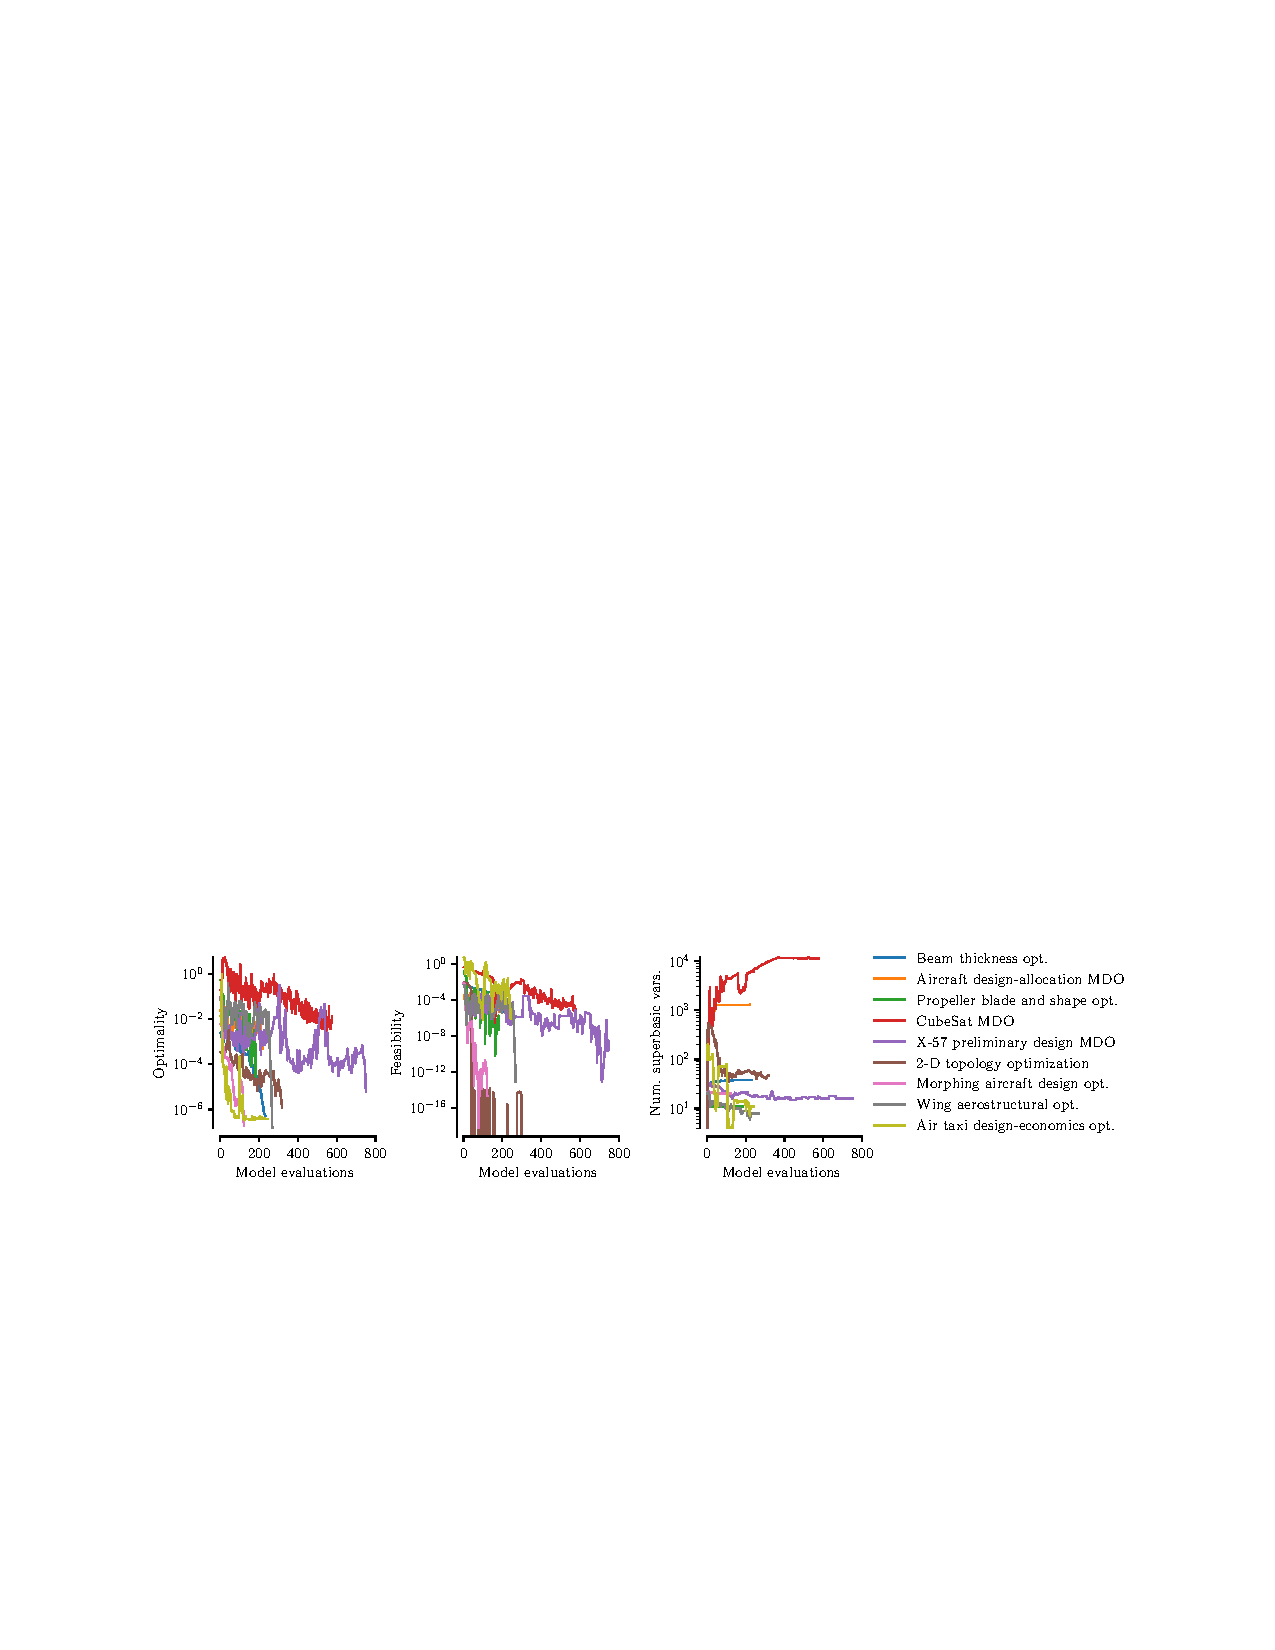
\includegraphics[width=\linewidth]{Figures/Figure1}
    \vspace{-5mm}
    % \caption{\textbf{The state-of-the-art in LSDO.}
    %     \normalfont{Previous LSDO problems}
    % }
    \label{fig:model_evals}
  \end{figure}
  \end{frame}


\subsection{State-of-the-art in LSDO: Challenges}
  \begin{frame}{State-of-the-art in LSDO: Challenges}
    \vspace{-10mm}
    \begin{itemize}
      \item Computational cost $\propto$ number of model evaluations
      \item Not fast enough to be adopted into an industrial setting
      \item OpenMDAO couples optimizers and models but both are still independent: Model acts as a black-box that outputs objective, constraints and their gradients
      \item A reduction in the number of model evaluations requires an intrusive approach where the internal components of the model are exposed to the optimizer
    \end{itemize}
    \vspace{1cm}
    \begin{figure}[ht]
      \centering
      \vspace{-15mm}
      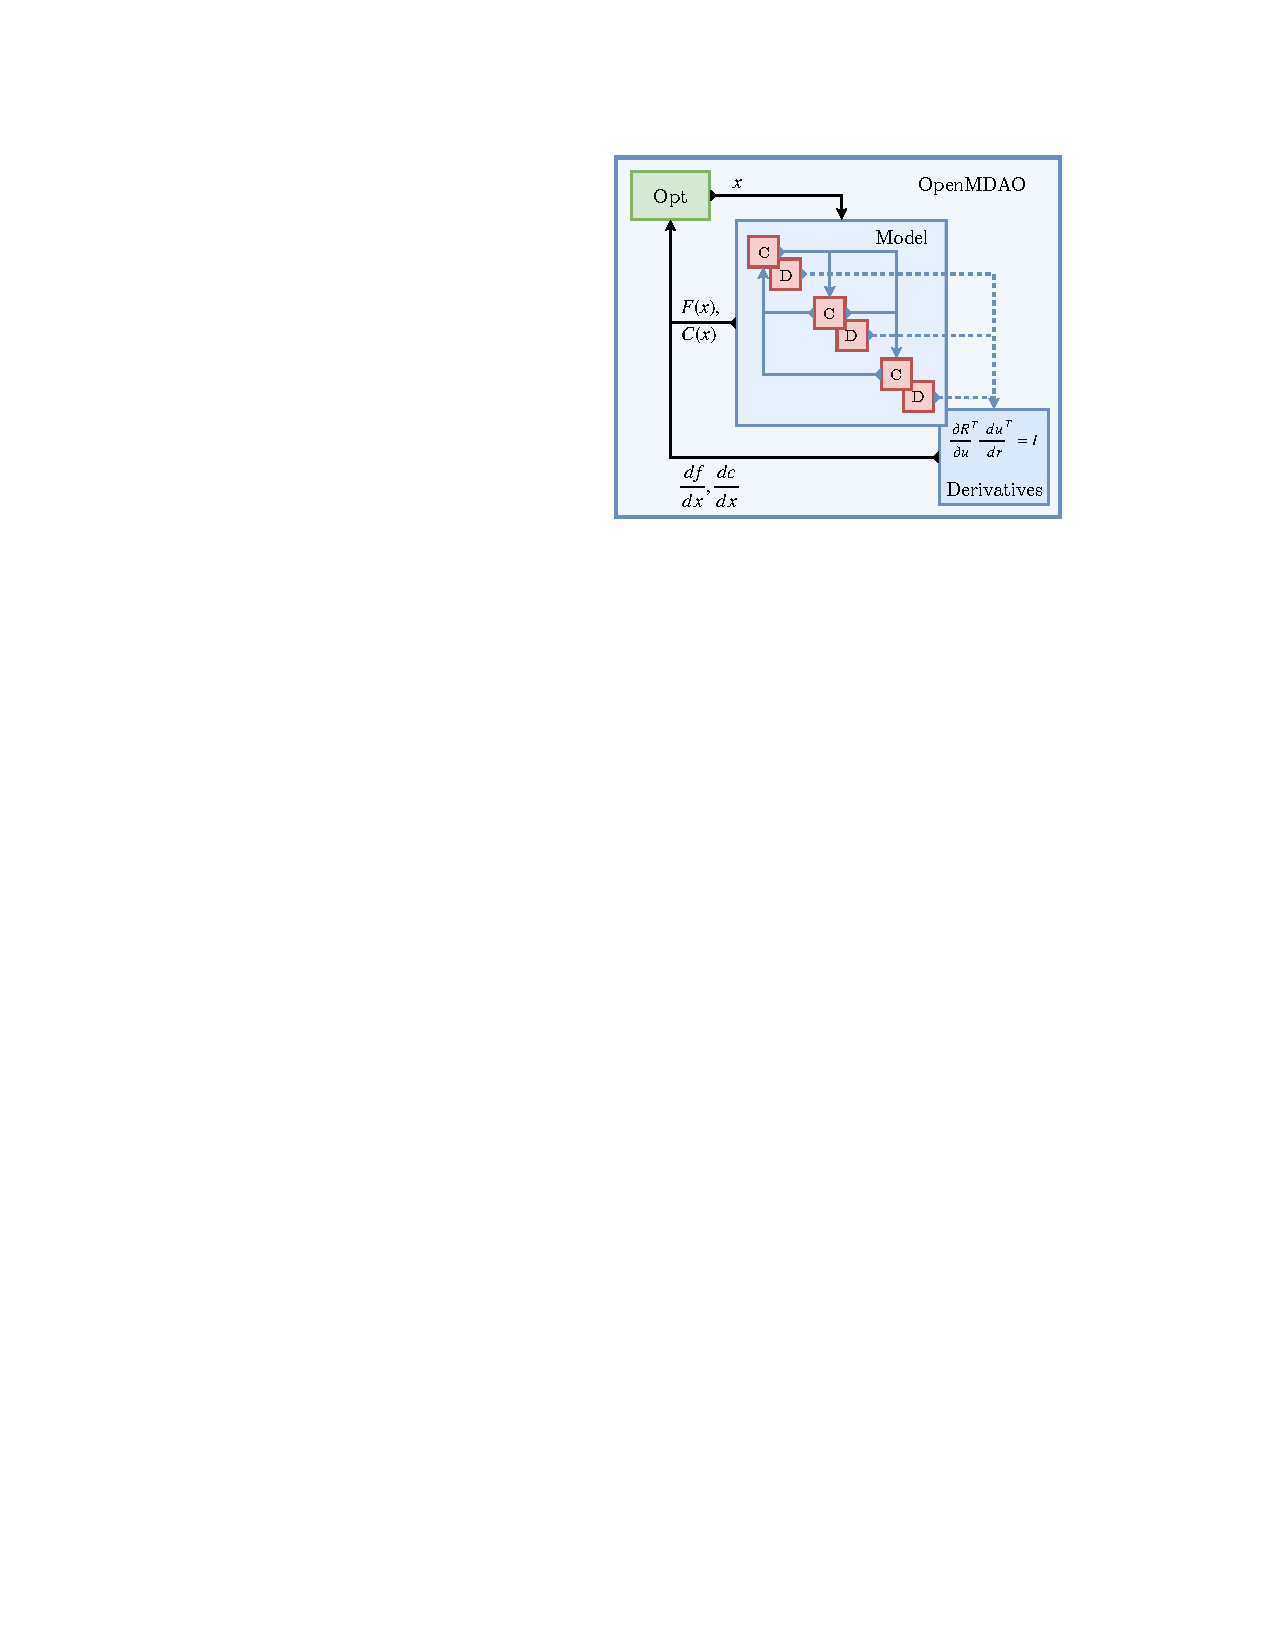
\includegraphics[width=.4\linewidth]{Figures/Figure5}
      \vspace{-5mm}
      % \caption{\textbf{The state-of-the-art in LSDO.}
      %     \normalfont{Previous LSDO problems}
      % }
      \label{fig:model_evals}
    \end{figure}
  \end{frame}


\section{Optimization Formulations}
  \begin{frame}[plain]
      \vfill
    \centering
    \begin{beamercolorbox}[sep=8pt,center,shadow=true,rounded=true]{title}
      \usebeamerfont{title}\insertsectionhead\par%
      \color{oxfordblue}\noindent\rule{10cm}{1pt} \\
      \LARGE{\faFileTextO}
    \end{beamercolorbox}
    \vfill
  \end{frame}


\subsection{Reduced-space method}
  \begin{frame}{Reduced-space method}
    Also known as multidisciplinary feasible(MDF) or nested analysis and design(NAND)
    \begin{figure}[ht]
      \centering
      \vspace{0mm}
      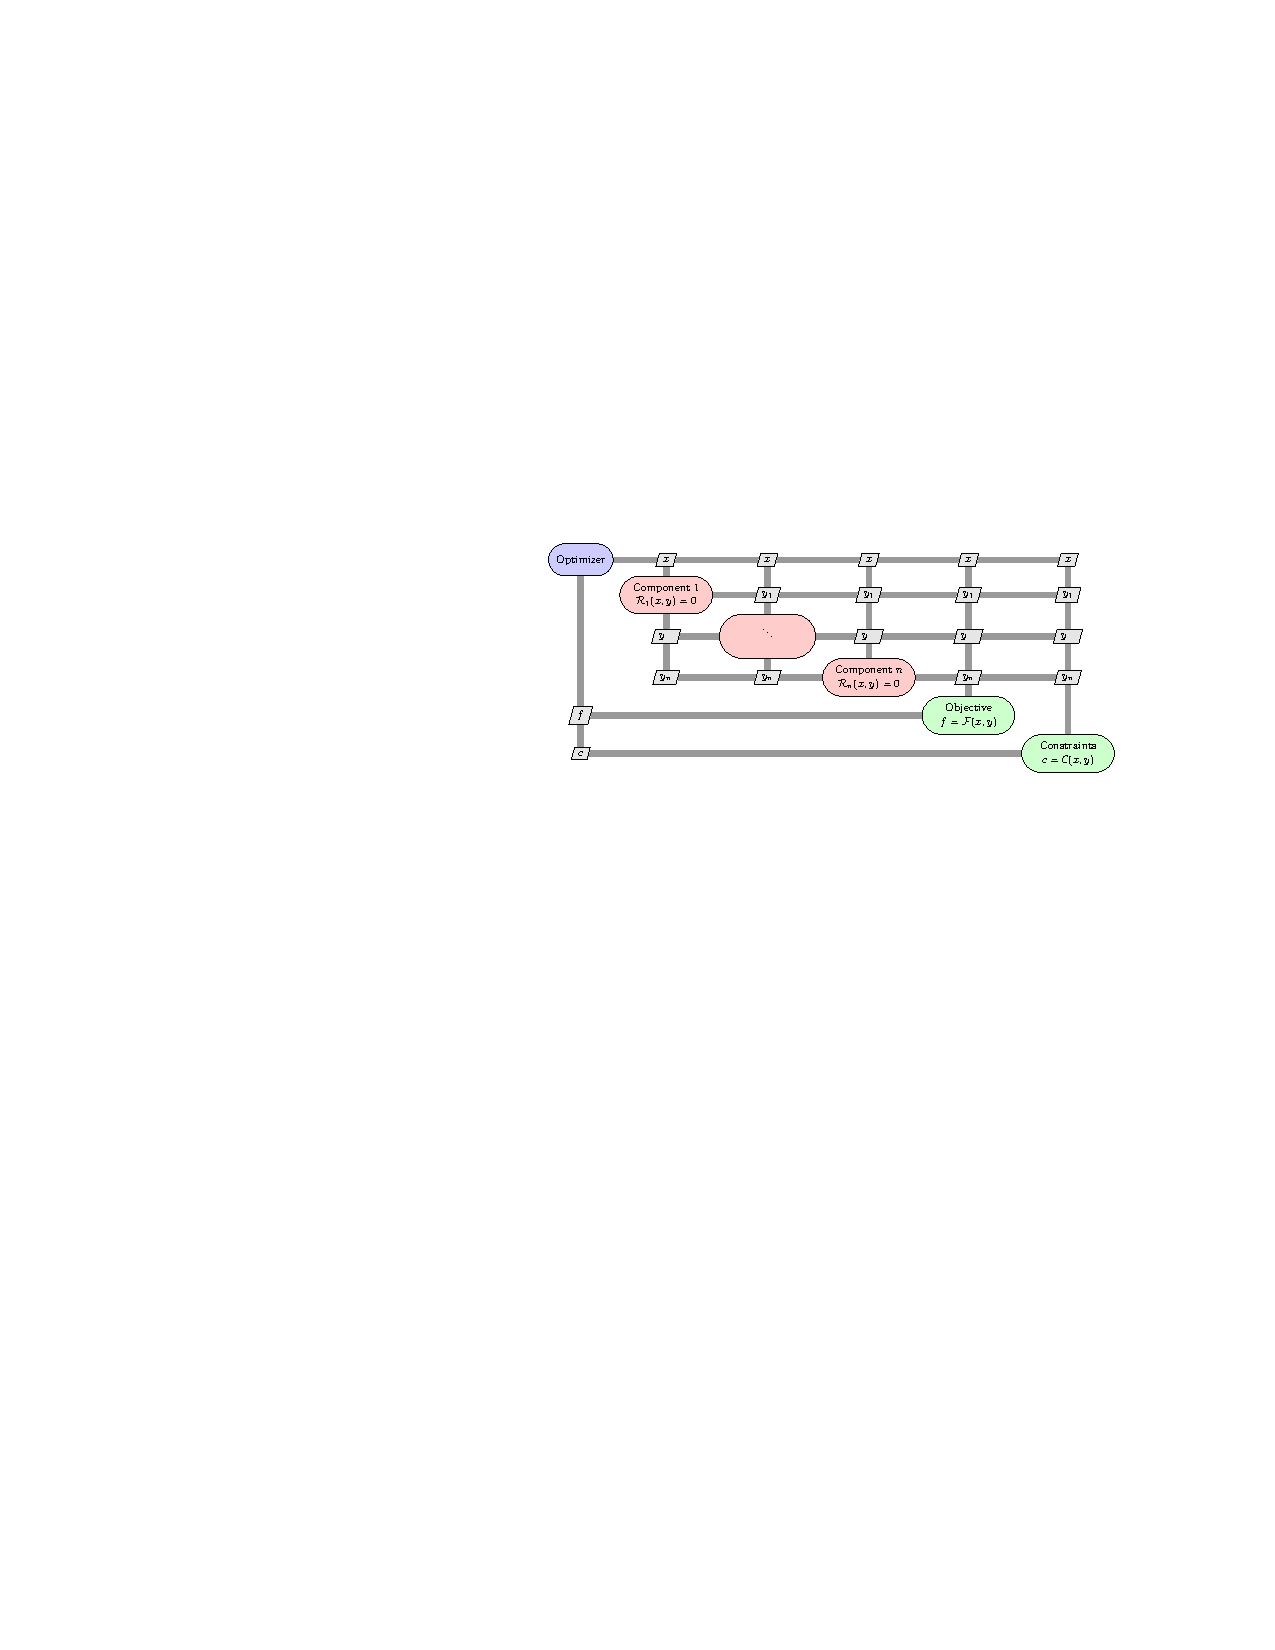
\includegraphics[width=.9\linewidth]{Figures/red_space}
      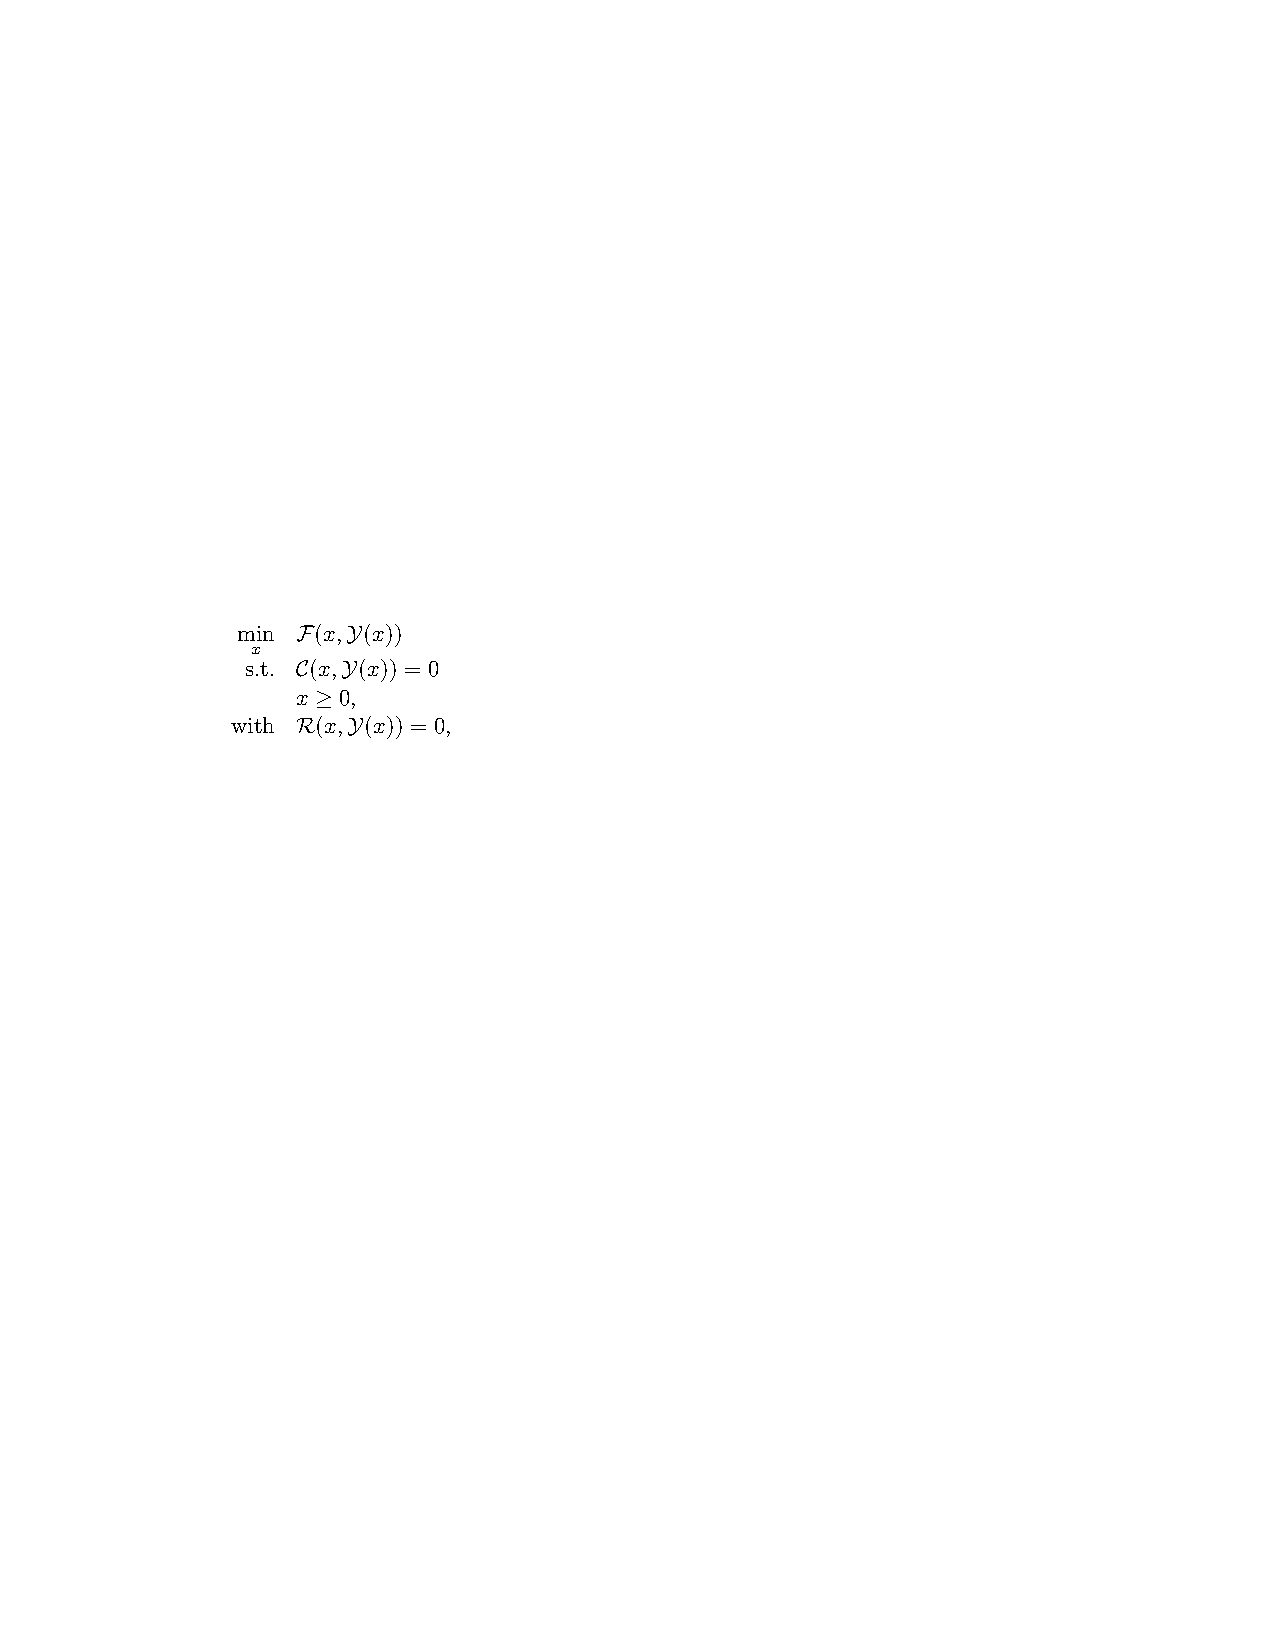
\includegraphics[width=.3\linewidth]{Figures/red_space_eqns}
      \vspace{-5mm}
      % \caption{\textbf{The state-of-the-art in LSDO.}
      %     \normalfont{Previous LSDO problems}
      % }
      \label{fig:model_evals}
    \end{figure}
  \end{frame}

  \begin{frame}{Reduced-space method}
    \vspace{-10mm}
    \begin{itemize}
      \item State variables corresponding to implicit equations are solved within the model.
      \item Non-linear solvers within a discipline will solve the residuals $R(x,y) = 0$ to compute $y$.
      \item Only $x$ constitutes the design variables and if $x \in \mathbb{R}^n$, the design space is $n$-dimensional and hence the name reduced-space.
    \end{itemize}
  \end{frame}

  \begin{frame}{RS: Optimality and KKT conditions}
    \vspace{-5mm}
    Define the Lagrangian as: 
    \vspace{2mm}
    \\ $l = \Ll(x, \lambda)$ where $\Ll(x, \lambda) = \F(x, \Y(x)) + \T{\lambda} \C(x, \Y(x))$ .
    \vspace{2mm}
    \\We obtain the following optimality conditions:
    \vspace{-1mm}
    \begin{equation*} %\tag{5}
        \begin{array}{l}
        \diff{l}{x} 
        % &= \diffp{\F}{x} + 
        % \left(
        %     -\diffp{\F}{y} \inv{\diffp{\R}{y}} - \lambda^T \diffp{\C}{y} \inv{\diffp{\R}{y}}
        % \right)
        % \diffp{\R}{x} + \lambda^T \diffp{\C}{x} \\
        = 
        \left( 
            \diffp{\F}{x} - \diffp{\F}{y} \inv{\diffp{R}{y}} \diffp{\R}{x}
        \right)
        + \lambda^T
        \left( 
            \diffp{\C}{x} - \diffp{\C}{y} \inv{\diffp{R}{y}} \diffp{\R}{x} 
        \right) \\
    
        \diff{l}{\lambda} = \C(x,\Y(x))
        
        \end{array}
        % \label{eq:rs_opt}
    \end{equation*}

    The KKT system is given by
    \begin{equation*} %\tag{6}
        \begin{bmatrix}
            l_{xx} &  \T{c_x} \\
             c_x  & 0\\
        \end{bmatrix}
        \begin{bmatrix}
            p_x \\
            p_{\lambda} \\
        \end{bmatrix}
        =
        \begin{bmatrix}
            -l_x \\ 
            -\C(x,\Y(x)) \\
        \end{bmatrix}
        ,
        % \label{eq:rs_kkt}
    \end{equation*}
    where $l_{xx} = d^2l/dx^2$, $c_x = dc/dx$, and $l_x = dl/dx$.
  \end{frame}

\subsection{Full-space method}
  \begin{frame}{Full-space method}
    Also known as simultaneous analysis and design(SAND)
    \begin{figure}[ht]
      \centering
      \vspace{0mm}
      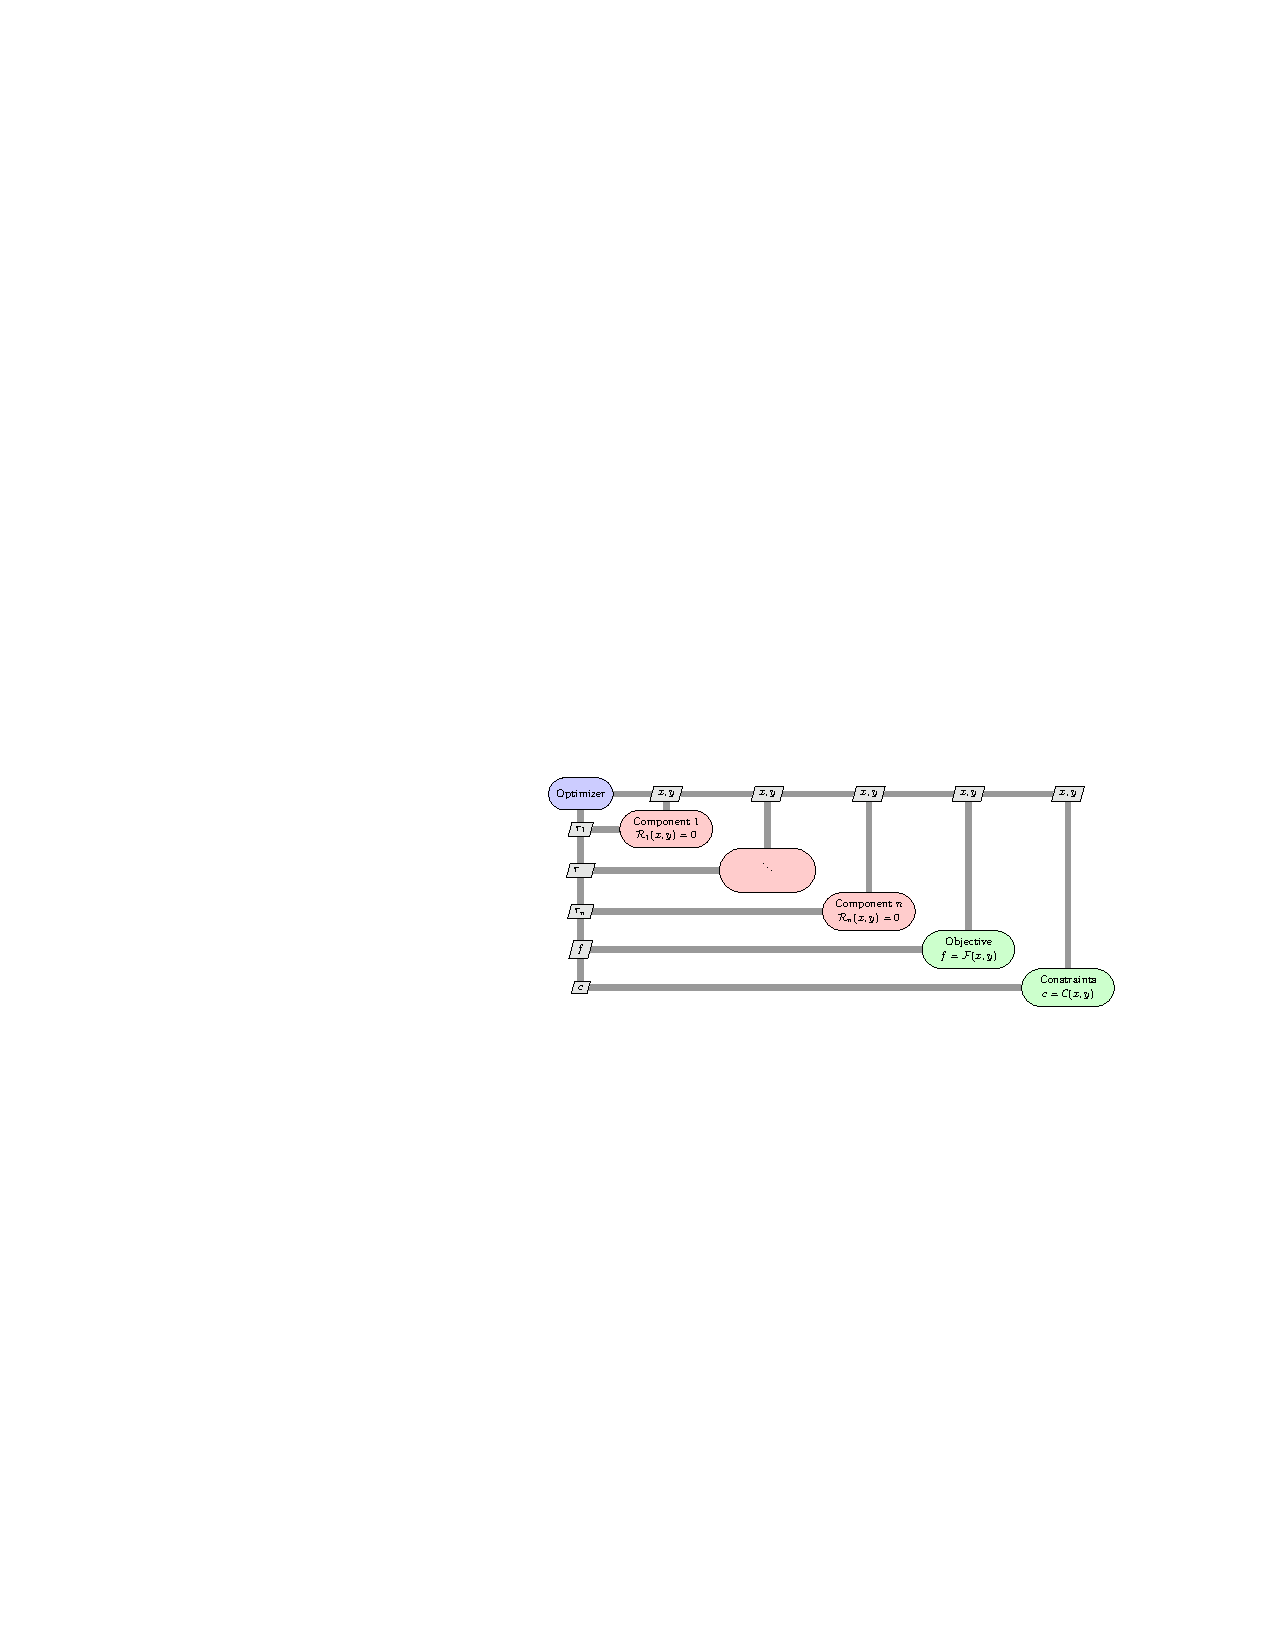
\includegraphics[width=.9\linewidth]{Figures/full_space}
      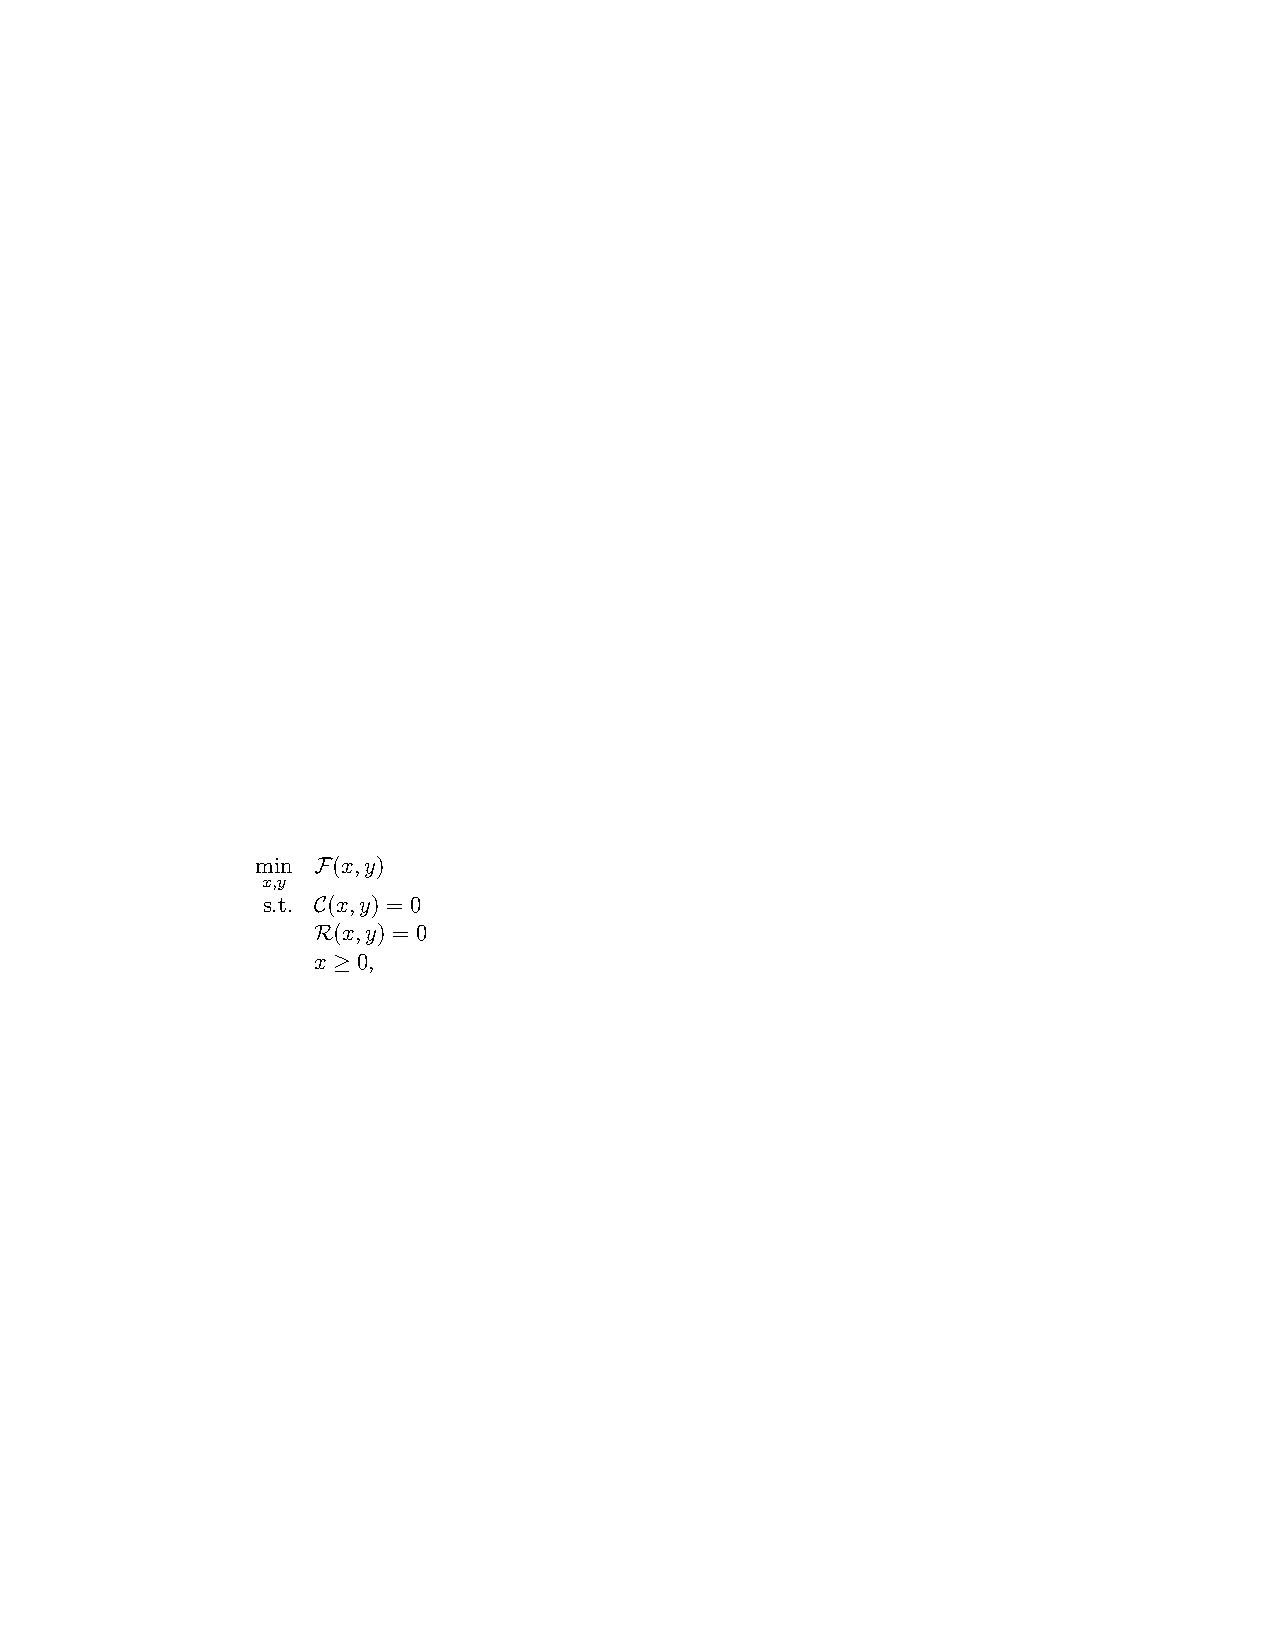
\includegraphics[width=.25\linewidth]{Figures/full_space_eqns}
      \vspace{-5mm}
      % \caption{\textbf{The state-of-the-art in LSDO.}
      %     \normalfont{Previous LSDO problems}
      % }
      \label{fig:model_evals}
    \end{figure}
  \end{frame}

  \begin{frame}{Full-space method}
    \vspace{-10mm}
    \begin{itemize}
      \item State variables corresponding to implicit equations are treated as design variables.
      \item Residuals $R(x,y) = 0$ are treated as additional constraints and the responsibilty of computing $y$ is on the optimizer.
      \item Both $x$ and $y$ constitutes the design variables and if $x \in \mathbb{R}^n$ and $y \in \mathbb{R}^k$, the design space is $(n + k)$-dimensional and hence the name full-space.
    \end{itemize}
  \end{frame}

  \begin{frame}{FS: Optimality and KKT conditions}
    Define the Lagrangian as:
    \vspace{2mm}
    \\ $m = \Mm(x, y, \psi, \lambda) = \F(x, y) + \T{\psi} \R(x,y) + \T{\lambda} \C(x,y)$. 
    \vspace{2mm}
    \\We obtain the following optimality conditions:
\begin{equation*} %\tag{7}
    \begin{array}{l l}
    \diff{m}{x} = \diffp{\F}{x} + \psi^T \diffp{\R}{x} + \lambda^T \diffp{\C}{x}
    & \diff{m}{\psi} = \R(x,y)\\
    \diff{m}{y} = \diffp{\F}{y} + \psi^T \diffp{\R}{y} + \lambda^T \diffp{\C}{y}
    & \diff{m}{\lambda} = \C(x,y)
    
    \end{array}
    \label{eq:fs_opt}
\end{equation*}
The KKT system is given by

\begin{equation*} %\tag{8}
    \begin{bmatrix}
        m_{xx} & m_{xy} &  \T{\R_x}  &  \T{\C_x} \\
        m_{yx} & m_{yy} &  \T{\R_y}  &  \T{\C_y} \\
         \R_x  &  \R_y & 0 & 0\\
         \C_x  &  \C_y & 0 & 0\\
    \end{bmatrix}
    \begin{bmatrix}
        p_x \\
        p_y \\
        p_{\psi} \\
        p_{\lambda} \\
    \end{bmatrix}
    =
    \begin{bmatrix}
        -m_x \\ 
        -m_y \\ 
        -\R(x,y) \\
        -\C(x,y) \\
    \end{bmatrix}
    \label{eq:fs_kkt}
\end{equation*}
% where $m_{xx} = d^2m/dx^2,~ m_{xy} = d^2m/dxdy, ~m_{yx} = d^2m/dydx,~  m_{yy} = d^2m/dy^2 ,~ \R_x = \partial\R/\partial x, ~\R_y = \partial\R/\partial y, ~\C_x = \partial\C/\partial x, ~\C_y = \partial\C/\partial y, ~m_x = dm/dx$  and $m_y = dm/dy$.
  \end{frame}

% \subsection{Reduced-space vs full-space}
  \begin{frame}{Reduced-space vs full-space}
    \begin{figure}[ht]
      \centering
      \vspace{0mm}
      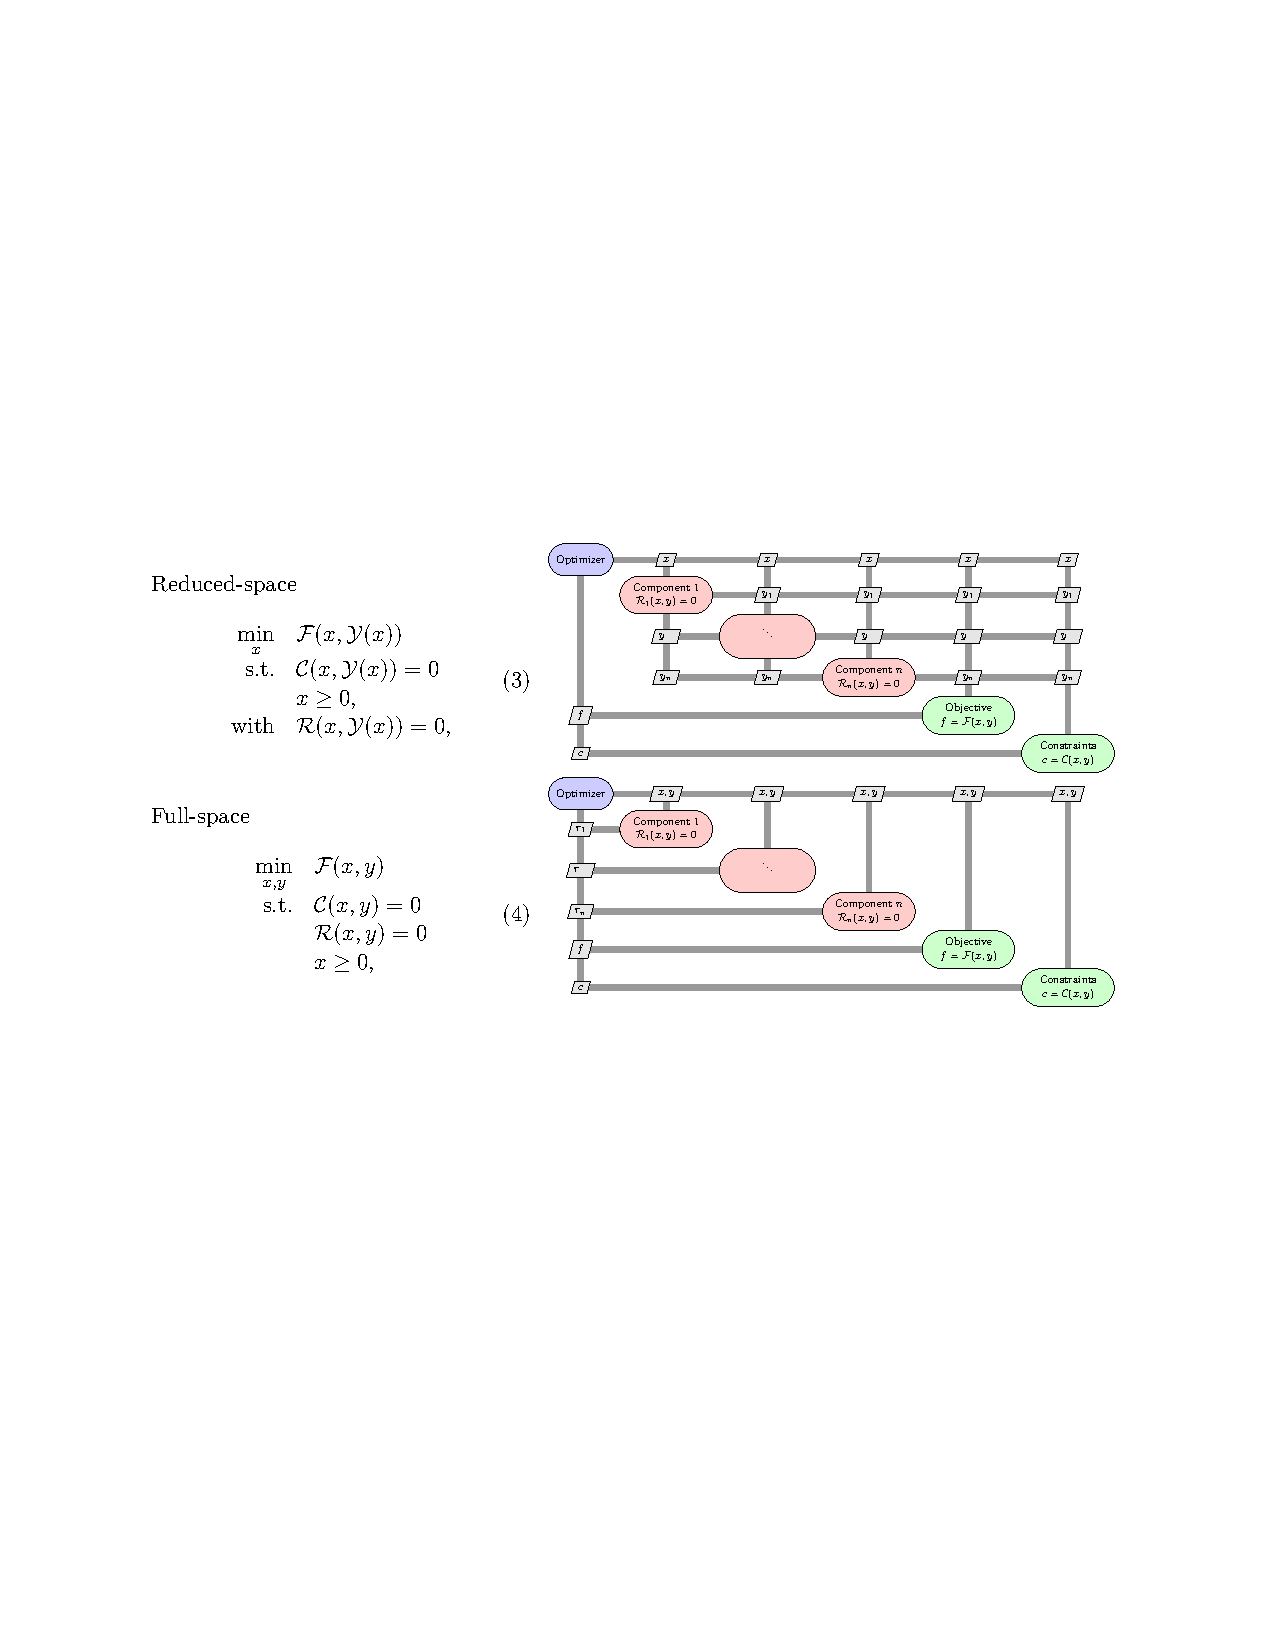
\includegraphics[width=.7\linewidth]{Figures/Figure2}
      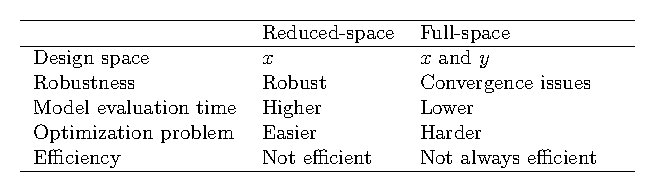
\includegraphics[width=.9\linewidth]{Figures/rs_vs_fs_table}
      \vspace{0mm}
      % \caption{\textbf{The state-of-the-art in LSDO.}
      %     \normalfont{Previous LSDO problems}
      % }
      \label{fig:model_evals}
    \end{figure}
  \end{frame}


\section{SURF - Strong Unification of Reduced-space and Full-space methods}
    \begin{frame}[plain]
        \vfill
      \centering
      \begin{beamercolorbox}[sep=8pt,center,shadow=true,rounded=true]{title}
        \usebeamerfont{title}\insertsectionhead\par%
        \color{oxfordblue}\noindent\rule{10cm}{1pt} \\
        \LARGE{\faFileTextO}
      \end{beamercolorbox}
      \vfill
  \end{frame}

  \begin{frame}{SURF: Basic Idea}
    \vspace{-10mm}
    \begin{itemize}
      \item State variables corresponding to implicit equations are solved to specified tolerances within the model.
      \item Solvers within a discipline will solve the residuals $R(x,y) \approx 0$ to compute an approximate $y$.
      \item $x$ constitutes the design variables and $y$ is a hybrid variable.
      \item A hybrid variable lies somewhere in the spectrum between a design variable and a state variable.
      \item Its location in the spectrum can be changed by adjustimg the solver tolerances. \\A zero tolerance on the non-linear solver is same as the reduce-space method while solving with infinite tolerance (equivalent to not solving $R(x,y) \approx 0$) in the same as a full-space method.
    \end{itemize}
  \end{frame}
  
  \begin{frame}{SURF: Algorithm}
    % \begin{algorithm}[ht]
    \small
    % \caption{Preliminary results: the SURF optimization algorithm}
    \caption{
        SURF (strong unification of reduced-space and full-space) \\ 
        \emph{SURF unifies reduced and full space for a simplified, equality-constrained optimization setting.}
    }
    \begin{algorithmic}[1]
        \Loop
            \State Assemble $A$, $b$, $\tilde M^{-1}$
            \State Solve $\tilde M^{-1} A p = \tilde M^{-1} b$
            \State Compute $\alpha$ via a line search
            \State Update $
                \begin{bmatrix}
                    x_+ ,
                    y_+ ,
                    \psi_+ ,
                    \lambda_+ 
                \end{bmatrix}^T
                =
                \begin{bmatrix}
                    x ,
                    y ,
                    \psi ,
                    \lambda 
                \end{bmatrix}^T
                + \alpha p
            $
            \State Update $y$ and $\psi$ by inexactly solving $\R(x,y)=0$ and
            % \State Update $y$ by inexactly solving $\R(x,y)=0$
            % \State Update $\psi$ by inexactly solving 
            % $\p \R / \p x ^ T \psi = -\p \F / \p y ^ T - \p \C / \p y ^ T \lambda$
            $\R_y^T \psi = -\F_y^T - \C_y^T \lambda$
            \State Update the approximation to the Hessian, ${d^2m/dx^2}$
        \EndLoop
    \end{algorithmic}

    \emph{Note}: 
    $p$ is the search direction and $\alpha$ is the step size,
    $Ap=b$ is the FS KKT system,
    and $M^{-1}$ and $\tilde M^{-1}$ are exact and approximate preconditioners for $A$ such that
    $M = M_1 M_2 M_3 M_4$ and
    % Schur-complement preconditioners for $A$:

    \begin{equation} %\tag{9}
        \setlength\arraycolsep{1pt}
        A =
        \begin{bmatrix}
            m_{xx} & m_{xy} & \T{\R_x} & \T{\C_x} \\
            m_{yx} & m_{yy} & \T{\R_y} & \T{\C_y} \\
            \R_x & \R_y & 0 & 0 \\
            \C_x & \C_y & 0 & 0 \\
        \end{bmatrix}
        ,
        b =
        \begin{bmatrix}
            -m_x \\ 
            -m_y \\ 
            -\R(x,y) \\ 
            -\C(x,y) \\
        \end{bmatrix}
        ,
        M_1 =
        \begin{bmatrix}
            0 & 0 & \I & 0 \\
            0 & \I & 0 & 0 \\
            \I & 0 & 0 & 0 \\
            0 & 0 & 0 & \I \\
        \end{bmatrix}
        ,
        M_2 =
        \begin{bmatrix}
            \R_y & 0 & 0 & 0 \\
            m_{yy} & \Tc{\R_y} & 0 & 0 \\
            m_{xy} & \Tc{\R_x} & \I & 0 \\
            \C_y & 0 & 0 & \I \\
        \end{bmatrix}
        % \label{eq:surf}
    \end{equation}
    
    \begin{equation}
        \setlength\arraycolsep{2pt}
        M_3 =
        \begin{bmatrix}
            \I & 0 & \invc{\R_y} \R_x & 0 \\
            0 & \I & \invTc{\R_y} m_{yx} - \invTc{\R_y} m_{yy} \invc{\R_y} \R_x & \invTc{\R_y} \Tc{\C_y} \\
            0 & 0 & 
            m_{xx} - m_{xy} \invc{\R_y} \R_x - \Tc{\R_x} \invTc{\R_y} m_{yx} + \Tc{\R_x} \invTc{\R_y} m_{yy} \invc{\R_y} \R_x
            & \Tc{\C_x} - \Tc{\R_x} \invTc{\R_y} \Tc{\C_y} \\
            0 & 0 & \C_x - \C_y \invc{\R_y} \R_x & 0 \\
        \end{bmatrix}
        ,
        M_4 =
        \begin{bmatrix}
            0 & \I & 0 & 0 \\
            0 & 0 & \I & 0 \\
            \I & 0 & 0 & 0 \\
            0 & 0 & 0 & \I \\
        \end{bmatrix}
        \nonumber
    \end{equation}

    % \begin{equation}
    %     \setlength\arraycolsep{3pt}
    %     A =
    %     \begin{bmatrix}
    %         m_{xx} & m_{xy} & \T{\R_x} & \T{\C_x} \\
    %         m_{yx} & m_{yy} & \T{\R_y} & \T{\C_y} \\
    %         \R_x & \R_y & 0 & 0 \\
    %         \C_x & \C_y & 0 & 0 \\
    %     \end{bmatrix}
    %     % \qquad \text{and} \qquad
    %     \; , \;
    %     b =
    %     \begin{bmatrix}
    %         -m_x \\ 
    %         -m_y \\ 
    %         -\R(x,\Y(x)) \\ 
    %         -\C(x,\Y(x)) \\
    %     \end{bmatrix}
    %     \; , \;
    % %     \qquad \text{and}
    % % \end{equation}
    % % \begin{equation}
    %     M =
    %     \underbrace{
    %         \begin{bmatrix}
    %             0 & 0 & \Id & 0 \\
    %             0 & \Id & 0 & 0 \\
    %             \Id & 0 & 0 & 0 \\
    %             0 & 0 & 0 & \Id \\
    %         \end{bmatrix}
    %     }_{M_1}
    %     \underbrace{
    %         \begin{bmatrix}
    %             \Ry & 0 & 0 & 0 \\
    %             \myy & \Tc{\Ry} & 0 & 0 \\
    %             \mxy & \Tc{\Rx} & \Id & 0 \\
    %             \Cy & 0 & 0 & \Id \\
    %         \end{bmatrix}
    %     }_{M_2}
    %     \nonumber
    % \end{equation}
    % \begin{equation}
    %     \setlength\arraycolsep{3pt}
    %     \underbrace{
    %         \begin{bmatrix}
    %             \Id & 0 & \invc{\Ry} \Rx & 0 \\
    %             0 & \Id & \invTc{\Ry} \myx - \invTc{\Ry} \myy \invc{\Ry} \Rx & \invTc{\Ry} \Tc{\Cy} \\
    %             0 & 0 & 
    %             \mxx - \mxy \invc{\Ry} \Rx - \Tc{\Rx} \invTc{\Ry} \myx + \Tc{\Rx} \invTc{\Ry} \myy \invc{\Ry} \Rx
    %             & \Tc{\Cx} - \Tc{\Rx} \invTc{\Ry} \Tc{\Cy} \\
    %             0 & 0 & \Cx - \Cy \invc{\Ry} \Rx & 0 \\
    %         \end{bmatrix}
    %     }_{M_3}
    %     \underbrace{
    %         \begin{bmatrix}
    %             0 & 0 & 0 & \Id \\
    %             \Id & 0 & 0 & 0 \\
    %             0 & 0 & \Id & 0 \\
    %             0 & \Id & 0 & 0 \\
    %         \end{bmatrix}
    %     }_{M_4}
    %     \label{eq:surf}
    % \end{equation}
    % \label{alg:surf}
\end{algorithm}
    \begin{figure}[ht]
      \centering
      \vspace{0mm}
      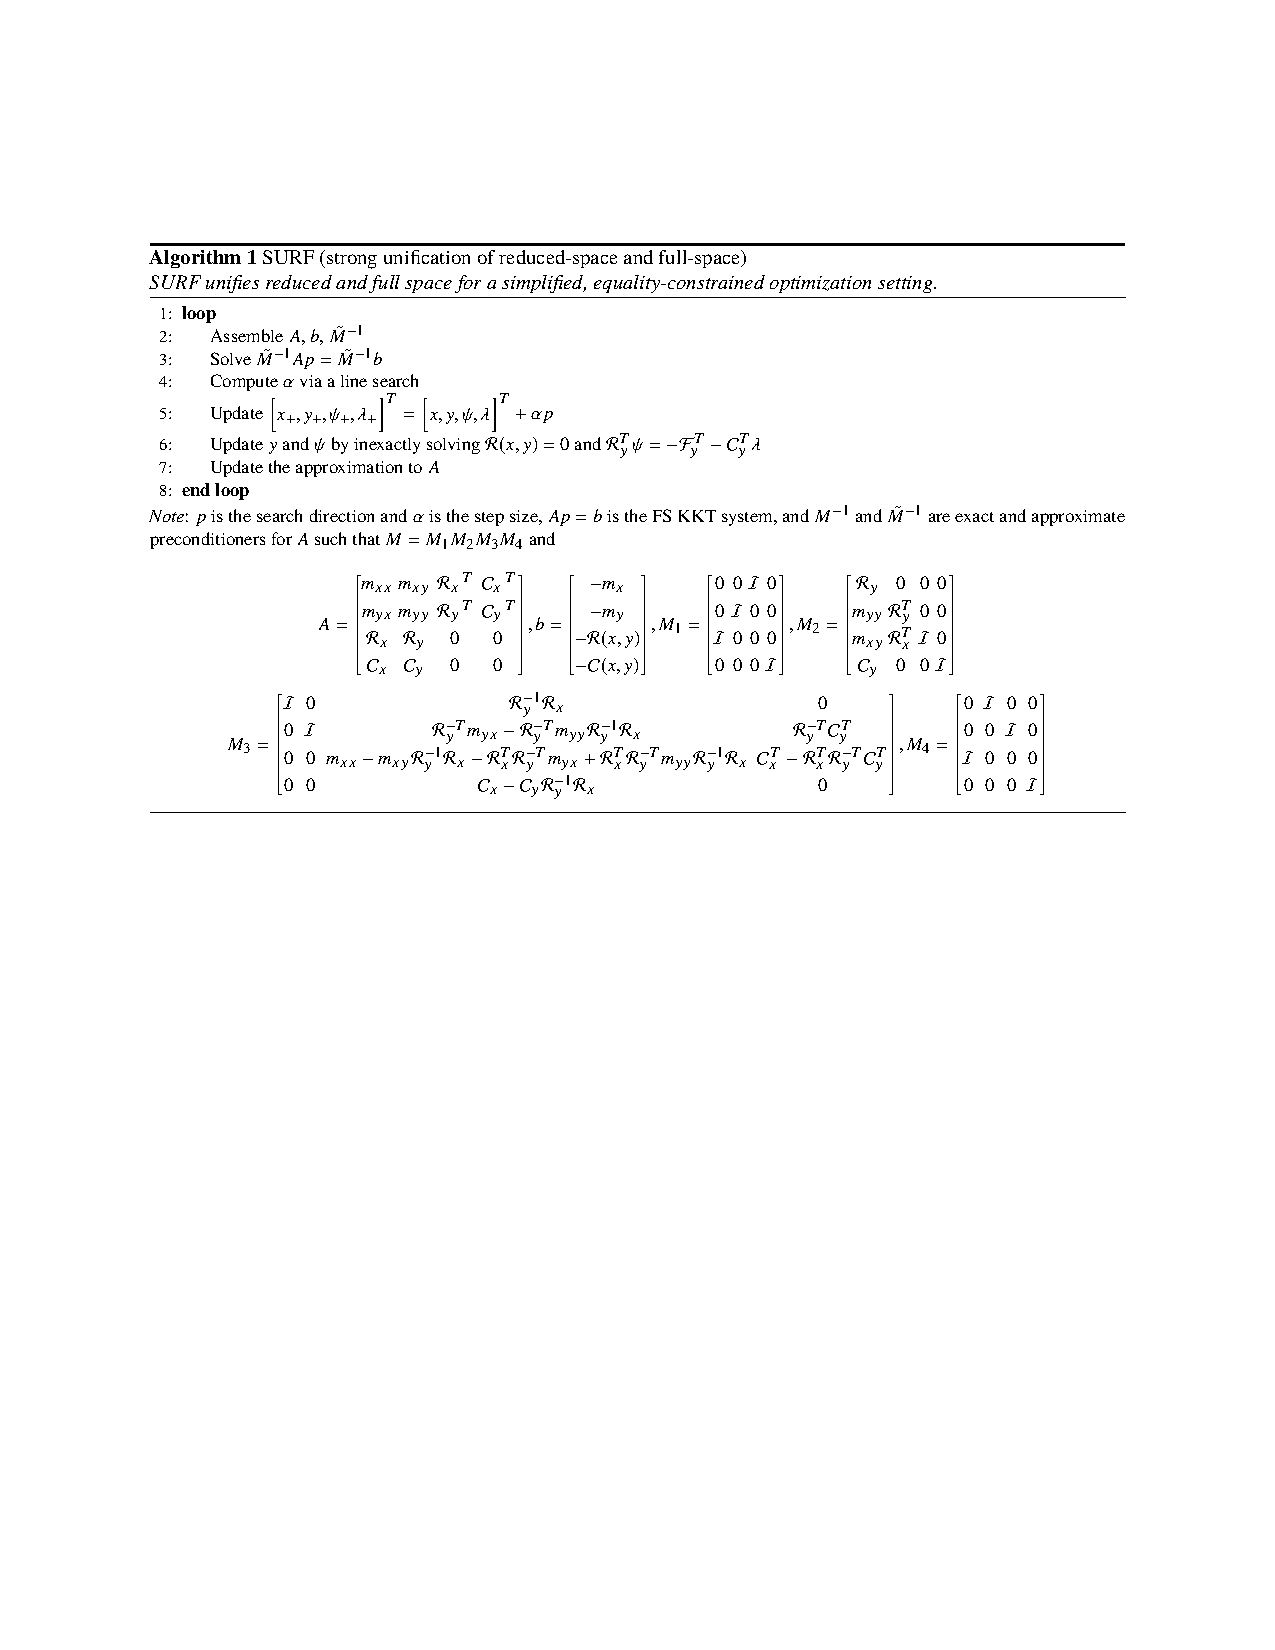
\includegraphics[width=\linewidth]{Figures/algorithm}
 
      % \caption{\textbf{The state-of-the-art in LSDO.}
      %     \normalfont{Previous LSDO problems}
      % }
      \label{fig:model_evals}
    \end{figure}
  \end{frame}
\subsection{SURF: Algorithm}
  \begin{frame}{SURF: Algorithm}
    \vspace{-10mm}
    \begin{itemize}
      \item Lines 2 and 3 represent the assembly and solution of the full-space KKT system with a preconditioner.
      \item Lines 4 and 5 computes the step size and applies the step.
      \item At this updated point, the non-linear system is solved inexactly and the value of y is updated again. Subsequently, we compute $\psi$ using an equation that comes from setting $dm/dy$ to zero. 
      
      \item Line 6 unifies the reduced space and full space formulations.
      \begin{itemize}
        \item If line 6 is skipped, SURF becomes a full space algorithm.
        \item If the two systems in line 6 are exactly solved SURF becomes a reduced space algorithm.
        \item If line 6 uses inexact solvers, SURF becomes a hybrid.
      \end{itemize}
      \item The equivalence of the full-space and reduced-space formulations are proven when the systems in line 6 are solved exactly.
    \end{itemize}
  \end{frame}

  \begin{frame}{SURF: Features}
    \vspace{-10mm}
    \begin{itemize}
      \item Switching between full-space and reduced-space is now simple.
      \item SURF allows easy access to a continuous spectrum of hybrid methods by just changing the inexact solver tolerances. 
      \item The choice on this spectrum can be made on a variable-by-variable basis.
    \end{itemize}
    \begin{figure}[ht]
      \centering
      \vspace{0mm}
      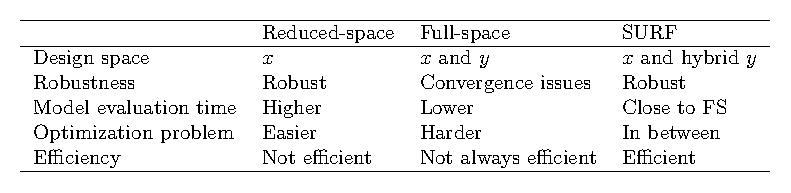
\includegraphics[width=\linewidth]{Figures/rs_vs_fs_vs_SURF_table}
      \vspace{0mm}
  \end{figure}
  \end{frame}

\subsection{SURF: FEA problem}
  \begin{frame}{SURF: FEA problem}
      \begin{itemize}
        \item SURF is applied to a beam thickness optimization problem
      
        \item The nonlinear, equality-constrained optimization problem is
          \begin{equation*} %\tag{14}
              \begin{array}{r l}
                  \min\limits_{x} & F^T d \\
                  \text{s.t.}
                  & V(x) = V_0 \\
                  % \text{governed by}
                  % & K(x, d) d - F = 0 , \\
              \end{array}
              \quad \text{with} \quad
              K(x, d) d - F = 0,
          \end{equation*}
   
        where $d$ is the displacement vector, $F$ is the force vector, $V(\cdot)$ is the volume function, $V_0$ is the allowable volume, and $K$ is the function that computes the stiffness matrix.
    
        
        \item The problem is solved using reduced-space and SURF optimizers.
        For SURF, we use pre-selected inexact solver tolerances.
    \end{itemize}
  \end{frame}

  \begin{frame}{SURF: FEA problem}

    \begin{figure}[ht]
        \centering
        \vspace{0mm}
        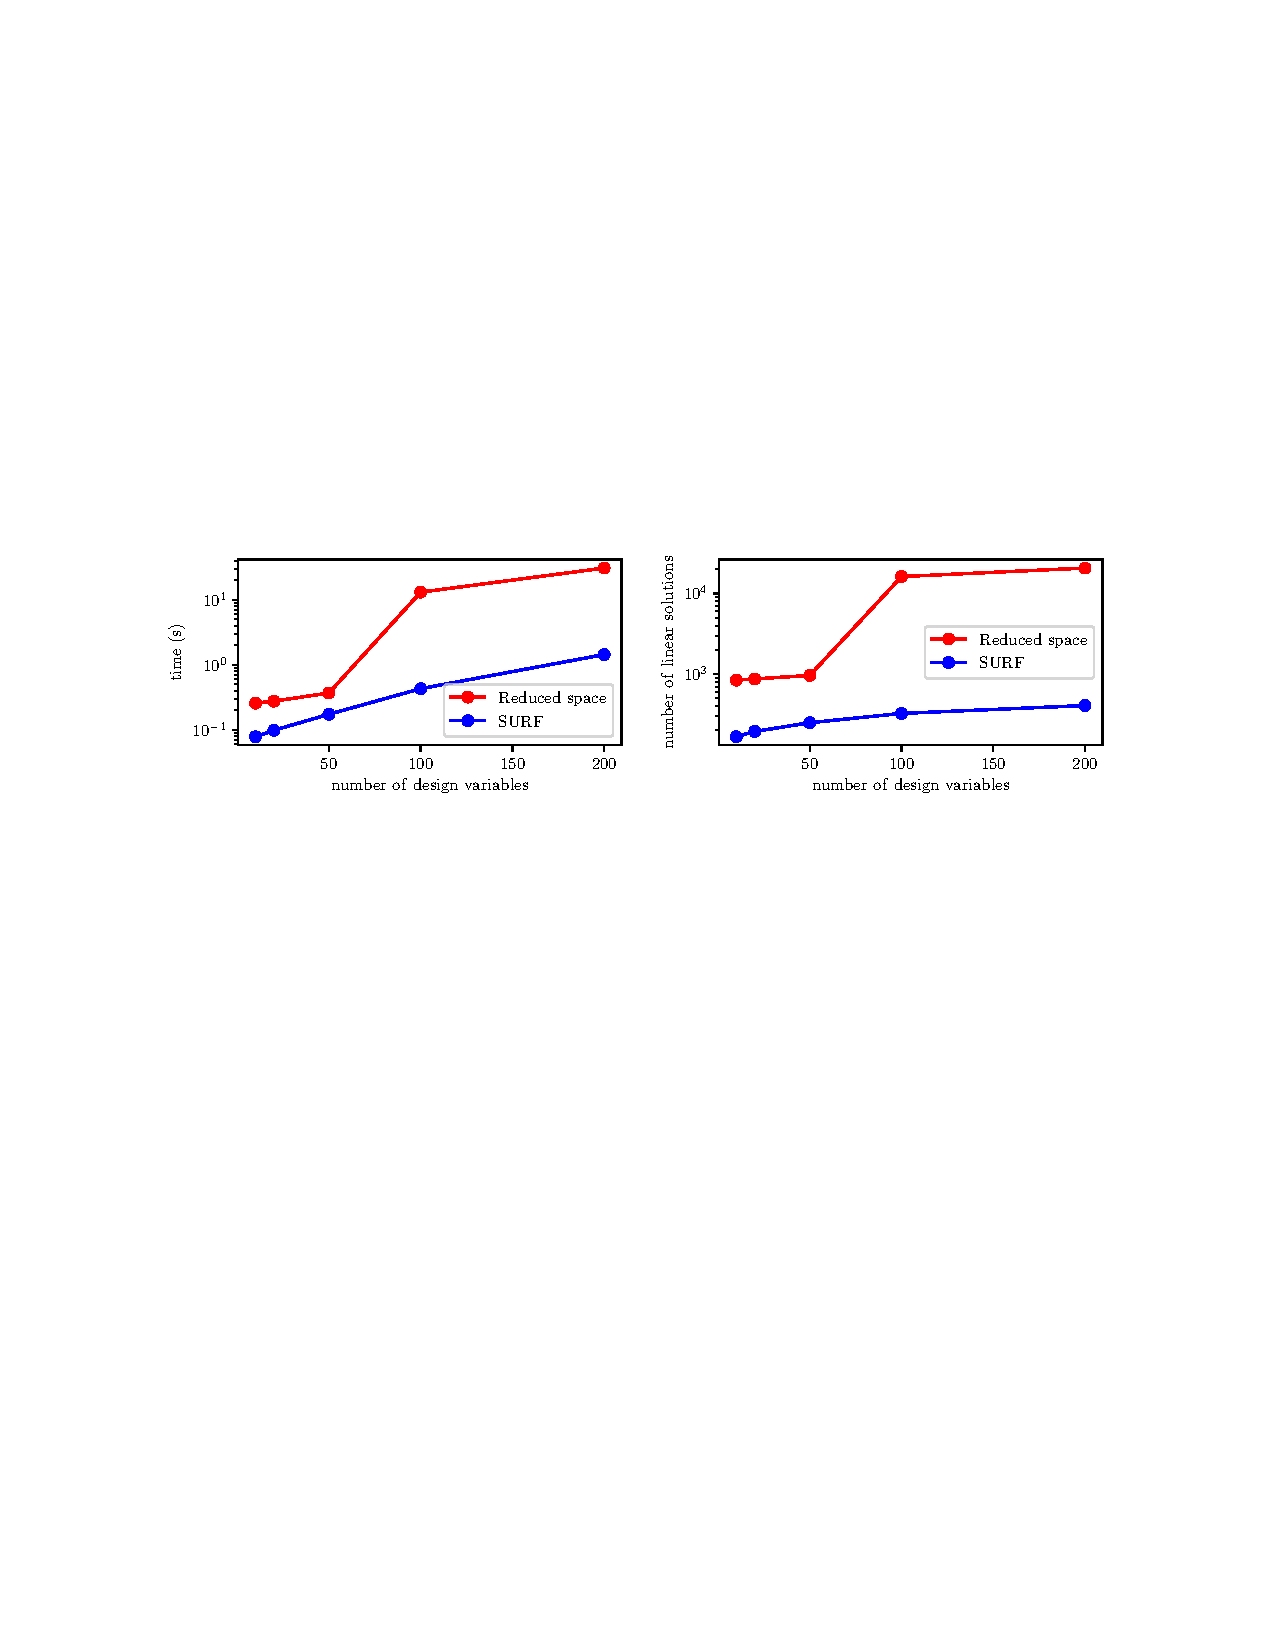
\includegraphics[width=\linewidth]{Figures/Figure3.pdf}
        \vspace{-5mm}
        % \caption{\textbf{Preliminary results.}
        %     \normalfont{On a scalable beam thickness optimization problem,
        %     the SURF algorithm is, on average, an order of magnitude more efficient than reduced-space optimization.}
        % }
        % \label{fig:preliminary}
    \end{figure}
    \begin{itemize}
      \item SURF with a hybrid formulation is, on average, an order of magnitude more efficient than the RS formulation in time and number of model evaluations across various numbers of beam elements.
    \end{itemize}
  \end{frame}

\section{Future work}
    \begin{frame}[plain]
        \vfill
      \centering
      \begin{beamercolorbox}[sep=8pt,center,shadow=true,rounded=true]{title}
        \usebeamerfont{title}\insertsectionhead\par%
        \color{oxfordblue}\noindent\rule{10cm}{1pt} \\
        \LARGE{\faFileTextO}
      \end{beamercolorbox}
      \vfill
  \end{frame}

  \begin{frame}{Future work}
    \vspace{-10mm}
    \begin{itemize}
      \item Extend the unification to inequality constrained optimization.
      \begin{itemize}
        \item Unification with active-set method
      \end{itemize} 
      \item Incorporating quasi-Newton updates into the SURF algorithm
      \begin{itemize}
        \item Unification with BFGS
      \end{itemize} 
      \item Adaptive hybrid selection - how to adaptively select solver tolerances during optimization.

    \end{itemize}
  \end{frame}

  
% \section{Questions}
  \begin{frame}[plain]
      \vfill
    \centering
    \begin{beamercolorbox}[sep=8pt,center,shadow=true,rounded=true]{title}
      \usebeamerfont{title}{Questions}\par%
      \color{oxfordblue}\noindent\rule{10cm}{1pt} \\
      \LARGE{\faFileTextO}
    \end{beamercolorbox}
    \vfill
  \end{frame}

% \subsection{Example}
% \begin{frame}{Example}
% \only<1>{
% Let \(p(x)=\mathcal{N}(\mu\textsubscript{1},\,\sigma^{2}\textsubscript{1})\) and \(q(x)=\mathcal{N}(\mu\textsubscript{2},\,\sigma^{2}\textsubscript{2})\): \\
% \begin{equation}
% \mathcal{N}=\frac{1}{\sigma\,\sqrt{2\,\pi}}\,\E^{-\frac{\left(x-\mu\right)^2}{2\,\sigma^2} }
% \end{equation}}
% \only<2>{
% Kullback-Leibler divergence for continuous probabilities:
% \begin{align*}
% 	D(p,q)=&\int p(x) \log \frac{p(x)}{q(x)}\ud x\\
%     =& \int p(x) \,\ln p(x) \ud x -\int p(x) \,\ln q(x) \ud x\\
% 	=&\,\frac{1}{2} \ln\left(2\,\pi\,\sigma_2^{2}\right) +\frac{\sigma_1^{2}+\left(\mu_1-\mu_2 \right)^2 }{2\,\sigma_2^2}-\frac{1}{2}\left( 1+\ln 2\,\pi\,\sigma_1^2\right) \\
% 	=&\,\ln\frac{\sigma_2}{\sigma_1} +\frac{\sigma_1^{2}+\left(\mu_1-\mu_2 \right)^2 }{2\,\sigma_2^2}-\frac{1}{2}
% \end{align*}
% }
% \end{frame}

% \section{Code}
%     \begin{frame}[plain]
%         \vfill
%       \centering
%       \begin{beamercolorbox}[sep=8pt,center,shadow=true,rounded=true]{title}
%         \usebeamerfont{title}\insertsectionhead\par%
%         \color{oxfordblue}\noindent\rule{10cm}{1pt} \\
%         \LARGE{\faFileCodeO}
%       \end{beamercolorbox}
%       \vfill
%   \end{frame}
  
% \subsection{Example}
% \begin{frame}[fragile]{Example}
% \begin{block}{Greatest Common Divisor}
% \begin{lstlisting}[firstnumber=1, label=glabels, xleftmargin=10pt] 
% def greatest_c_remainder(a,b):
% 	'''Greatest common divisor of a and b'''
% 	r = a % b
% 	if r == 0:
% 		return b
% 	else:
% 		m = b
% 		n = r
% 	return greatest_c_remainder(m,n)

% \end{lstlisting}
% \end{block}
% \end{frame}
\endgroup


\end{document}

